\chapter{Input and output}

A number of years ago, Jeannette Wing published a terrific editorial with the title {\it Computational Thinking}, or in her own words, ``Ways to Think Like a Computer Scientist'' (see Communications of the ACM, March 2006).
This 3-page article summarizes many of the problem-solving techniques you will discover while learning to program.
Everyone interested in learning computer science beyond programming should read it.
She defines the field this way:

\begin{quote}
{\bf ``Computer science is the study of computation---what can be computed and how to compute it.''}
\end{quote}

So far the only programs we've looked at simply display messages, which doesn't involve a lot of real computation.
But that will change quickly as we begin to work with more types of data.
This chapter will show you how to read input from the keyboard, use that input to calculate a result, and then format that result for output.
We will also look at some technical details about how operating systems work.


\section{Packages}

\index{library}

Like most programming languages, Java has an extensive {\bf library} of class and method definitions that you can use in your programs.
You can browse this library on Oracle's website:
\url{http://docs.oracle.com/javase/7/docs/api/}

\index{package}

The standard edition of Java comes with {\em several thousand} classes, which can be both exciting and intimidating.
To help keep things organized, classes are grouped into {\bf packages}.
Just like each class is a separate file, each package is a separate folder.

\begin{figure}[h!]
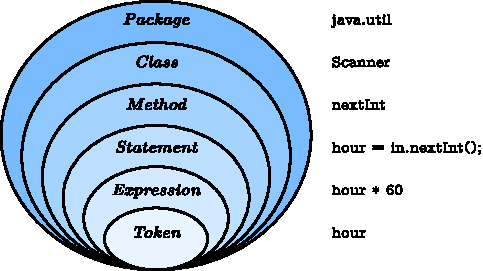
\includegraphics[width=4in]{package.pdf}
\caption{Elements of the Java language, from largest to smallest.}
\end{figure}

Two library classes we have seen thus far, \java{System} and \java{String}, belong to the \java{java.lang} package. According to the documentation, \java{java.lang} ``provides classes that are fundamental to the design of the Java programming language.''
Note there is a major difference between the Java {\em language}, which deals with syntax and grammar, and the Java {\em library}, which provides the built-in classes.
In fact, the Java library itself is written in Java!

\index{import}
\index{statement!import}

In order to use a class defined in another package (and in another folder), you have to {\bf import} it first:

\begin{code}
import java.io.File;
import java.io.PrintStream;
import java.util.Date;
import java.util.Scanner;
\end{code}

All \java{import} statements appear at the beginning of the source file, above the class definition.
It's not uncommon for Java programs to have dozens of import statements.
Because they are so fundamental, all classes in \java{java.lang} are imported automatically.
That is why we haven't needed the \java{import} statement until now.


\section{The System class}
\label{system}

\index{System class}
\index{class!System}
\index{object}

When you call \java{System.out.println}, you are referring to the \java{out} variable declared in the \java{System} class.
The \java{out} variable's type is \java{PrintStream}, which provides methods for ``printing'' data.
Both \java{System} and \java{PrintStream} are written in Java, and later in the book we'll examine their source code.
For now, you should understand that \java{System.out} is an {\bf object} of type \java{PrintStream}.
Because Java is an {\em object-oriented} language, much of the library is organized around objects rather than methods.

\begin{figure}[h!]
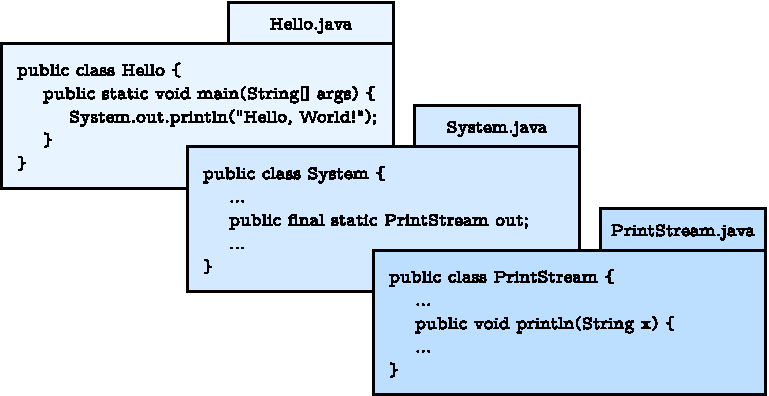
\includegraphics{system.pdf}
\caption{\java{System.out.println} references the \java{out} variable of the \java{System} class,
\\ which has the type \java{PrintStream}, which has a method called \java{println}.}
\end{figure}

\index{operating system}

Java programs run on top of an {\bf operating system} that manages the keyboard, the display, main memory, disk drives, the network, and other hardware resources.
Common examples of operating systems include Android, iOS, Linux, Mac OS~X, and Windows.
When starting Java programs, the operating system directs \java{System.out} to the screen.

You can even use \java{System.out} to print \java{System.out}:

\begin{code}
System.out.println(System.out);
\end{code}

The result is:

\begin{stdout}
java.io.PrintStream@685d72cd
\end{stdout}

\index{address}

When Java prints an object, it prints the type of the object (\java{PrintStream}), the package where the type is defined (\java{java.io}), and the {\bf address} or location of the object in memory.
In this example the address is \java{685d72cd}, but if you run the same code you will most likely get something different.
You can think of the address as a unique identifier for the object.

\index{abstraction}

Note the exact type of display doesn't matter, whether it's a 5-inch touch screen or 30-inch monitor.
From the programmer's point of view, \java{System.out} simply provides the means for displaying messages.
Computer scientists often use {\bf abstraction} to deal with the complexity of software.
The \java{System} class is a platform-independent abstraction of the operating system.
The operating system itself is a layer of abstraction on top of computer hardware.

There is also an object named \java{System.in} that makes it possible to get input from the keyboard.
As with \java{System.out}, the exact type of keyboard (or touch screen) does not matter to the programmer.
Unfortunately, Java does not make it easy to use \java{System.in} directly.
Instead, it provides other classes that make use of \java{System.in} for you.


\section{The Scanner class}

\index{byte}

From the operating system's point of view, data from the keyboard arrives in a series of hardware control signals.
The operating system translates these signals into a stream of \textbf{bytes} (small integers), which in turn need to be translated into characters.
\java{System.in} provides the means for reading one byte of input at a time, which is hardly useful for programs that would rather read in an entire word or line of input.

\index{class!utility}
\index{utility class}

That's where \java{java.util.Scanner} comes in handy.
\java{Scanner} is a {\bf utility class} that parses an input stream into words, lines, numbers, and other types of data.
Because \java{Scanner} belongs to the \java{java.util} package, you need to import it at the top of your program.
Otherwise you will get a compiler error like ``cannot find symbol'' (i.e., the compiler doesn't know what you mean by \java{Scanner}).

\begin{code}
import java.util.Scanner;
\end{code}

In most programs, you will need only one \java{Scanner}, since there is only one source of input.
The following code first declares a \java{Scanner} variable, and then creates a \java{Scanner} object that scans \java{System.in}.

\begin{code}
    Scanner in;
    in = new Scanner(System.in);
\end{code}

\index{initialize}

As we saw previously with constants, it is also legal to declare a variable and initialize it at the same time:

\begin{code}
    Scanner in = new Scanner(System.in);
\end{code}

This latter syntax is more convenient, since it's a one-time setup for many programs.
Just make sure you understand that it's two statements in one.

At this point, you can use the variable \java{in} instead of \java{System.in}.
The following example reads two lines of input from the keyboard and repeats them back again to the user.

\begin{code}
import java.util.Scanner;

public class Echo {

    public static void main(String[] args) {
        String line;
        Scanner in = new Scanner(System.in);

        System.out.print("Type something:");
        line = in.nextLine();
        System.out.println("You said: " + line);

        System.out.print("Type something else:");
        line = in.nextLine();
        System.out.println("You also said: " + line);
    }

}
\end{code}


\section{Reading documentation}
\label{documentation}

\index{documentation}

Now would be a good time to take a look at the documentation for \java{Scanner}.
You can find it from the Java library (see the link earlier in this chapter) or simply do a web search for ``java scanner.''
The latter method is more useful in the long run, especially as versions of Java change.
Either way, you should get something like this:

\begin{figure}[h!]
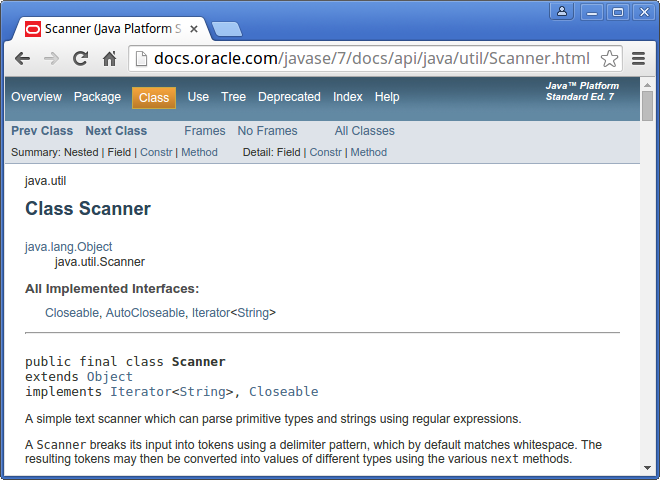
\includegraphics[width=\textwidth]{scanner.png}
\caption{Screenshot of the documentation for \java{Scanner} on Oracle's website.}
\end{figure}

Scroll down to the ``Method Summary'' section.
As you can see, the \java{Scanner} class provides quite a few methods.
In this chapter we'll focus on the ``next'' methods.
For example, click on the link for \java{nextInt}.

\begin{stdout}
public int nextInt()

Scans the next token of the input as an int.
\end{stdout}

\index{prototype}

The first line is the method's {\bf prototype}, which specifies the name of the method and the return type.
In this example, \java{nextInt} returns an \java{int}.
The next line describes what the method does.
The following lines explain the parameters (if any) and return values.
The explanations are often redundant, but the documentation is supposed to fit a standard format.
%The last line describes the exceptions this method might throw.

It might take some time to get comfortable reading this kind of information, but it's well worth the effort.
Knowing what methods a class provides helps you avoid reinventing the wheel.
Whenever you learn about a new class, you should take a quick look at its documentation.
In fact, take a few minutes and look at the docs for \java{System} and \java{String}.


\section{The modulus operator}
\index{modulus}
\index{operator!modulus}

The modulus operator works on integers (and integer expressions) and yields the {\em remainder} when the first operand is divided by the second.
In Java, the modulus operator is a percent sign, {\tt \%}.
The syntax is the same as for other operators:

\begin{code}
    int quotient = 7 / 3;
    int remainder = 7 % 3;
\end{code}

The first operator, integer division, yields 2.
The second operator yields 1.
Thus, 7 divided by 3 is 2 with 1 left over.

The modulus operator turns out to be surprisingly useful.
For example, you can check whether one number is divisible by another: if {\tt x \% y} is zero, then {\tt x} is divisible by {\tt y}.

Also, you can use the modulus operator to extract the rightmost digit or digits from a number.
For example, {\tt x \% 10} yields the rightmost digit of {\tt x} (in base 10).
Similarly {\tt x \% 100} yields the last two digits.


\section{Floating-point numbers}
\index{floating-point}
\index{type!double}
\index{double(floating-point)}

In the last chapter we had some problems dealing with numbers that were not integers.
We worked around the problem by measuring percentages instead of fractions, but a more general solution is to use floating-point numbers, which can represent fractions as well as integers.
In Java, the floating-point type is called {\tt double}, which is short for ``double-precision.''

You can create floating-point variables and assign values to them using the same syntax we used for the other types.
For example:

\begin{code}
    double pi;
    pi = 3.14159;
\end{code}

It is also legal to declare a variable and assign a value to it at the same time:

\begin{code}
    int x = 1;
    String empty = "";
    double pi = 3.14159;
\end{code}

\index{initialization}

This syntax is common; a combined declaration and assignment is sometimes called an {\bf initialization}.

Although floating-point numbers are useful, they are a source of confusion because there seems to be an overlap between integers and floating-point numbers.
For example, if you have the value {\tt 1}, is that an integer, a floating-point number, or both?

Java distinguishes the integer value {\tt 1} from the floating-point value {\tt 1.0}, even though they seem to be the same number.
They belong to different types, and strictly speaking, you are not allowed to make assignments between types.
For example, the following is illegal:

\begin{code}
    int x = 1.1;
\end{code}

because the variable on the left is an {\tt int} and the value on the right is a {\tt double}.
But it is easy to forget this rule, especially because there are places where Java will automatically convert from one type to another.

For example:

\begin{code}
    double y = 1;
\end{code}

should technically be illegal, but Java allows it by converting the {\tt int} to a {\tt double} automatically.
This leniency is convenient, but it can cause problems; for example:

\begin{code}
    double y = 1 / 3;
\end{code}

You might expect the variable {\tt y} to get the value {\tt 0.333333}, which is a legal floating-point value, but in fact it gets {\tt 0.0}.
The reason is that the expression on the right is the ratio of two integers, so Java does {\em integer} division, which yields the integer value {\tt 0}.
Converted to floating-point, the result is {\tt 0.0}.

One way to solve this problem (once you figure out what it is) is to make the right-hand side a floating-point expression:

\begin{code}
    double y = 1.0 / 3.0;
\end{code}

This sets {\tt y} to {\tt 0.333333}, as expected.

\index{arithmetic!floating-point}

The operations we have seen so far---addition, subtraction, multiplication, and division---also work on floating-point values, although you might be interested to know that the underlying mechanism is completely different.
In fact, most processors have special circuitry just for performing floating-point operations.


\section{Converting from double to int}
\label{rounding}
\index{rounding}
\index{typecasting}

As I mentioned, Java converts {\tt int}s to {\tt double}s automatically if necessary, because no information is lost in the translation.
On the other hand, going from a {\tt double} to an {\tt int} requires rounding off.
Java doesn't perform this operation automatically, in order to make sure that you, as the programmer, are aware of the loss of the fractional part of the number.

The simplest way to convert a floating-point value to an integer is to use a {\bf typecast}.
Typecasting is so called because it allows you to take a value that belongs to one type and ``cast'' it into another type (in the sense of molding or reforming).

The syntax for typecasting is to put the name of the type in parentheses and use it as an operator.
For example:

\begin{code}
    double pi = 3.14159;
    int x = (int) pi;
\end{code}

The {\tt(int)} operator has the effect of converting what follows into an integer, so {\tt x} gets the value 3.

Typecasting takes precedence over arithmetic operations, so in the following example, the value of {\tt pi} gets converted to an integer first, and the result is 60.0, not 62.

\begin{code}
    double pi = 3.14159;
    double x = (int) pi * 20.0;
\end{code}

Converting to an integer always rounds down, even if the fraction part is 0.99999999.
These behaviors (precedence and rounding) can make typecasting error-prone.


\section{Escape characters}

TODO


\section{Formatting output with printf}

TODO


\section{Putting it all together}

TODO


\section{Testing via the command line}

TODO
